\documentclass[output=paper]{langsci/langscibook}

\author{Adam Ledgeway\affiliation{University of Cambridge}}
\title{Rethinking microvariation in Romance demonstrative systems}

% \chapterDOI{} %will be filled in at production

\abstract{This article explores the formal and functional organization of
    \ili{Romance} demonstrative\is{demonstratives} systems, providing a detailed empirical overview of
    the vast \isi{microvariation} attested in standard and non-standard \ili{Romance}
    varieties. Despite highlighting a considerable number of distinct
    demonstrative\is{demonstratives} systems based on different superficial person contrasts, it
    is argued that the underlying number of systems can effectively be reduced
    to a much smaller number of systems based on a finite number of options. In
    particular, it is argued that the feature geometric analysis of person
    developed by \citet{HarRit2002} makes some specific predictions about the
    range and types of person combinations, and hence by implication also the
    types and natural classes of demonstrative\is{demonstratives} systems, that are
    cross-linguistically available. Adopting these assumptions, it is argued
    that these differing person feature specifications can be profitably
    modelled in terms of a set of hierarchically-organized interrelated
    parametric options in accordance with much recent work developed within the
ReCoS group.}

\maketitle

\begin{document}\glsresetall

\section{Introduction and general remarks}\label{sec:1}

Traditional descriptions of \ili{Romance} demonstrative\is{demonstratives} systems highlight a major
distinction between binary (cf.\ \ref{ex:08.1}a below) and ternary (cf.\
\ref{ex:08.1}b below) person-based systems (cf.\
\citealt[645--647]{Meyer-Lubke:1895a}; \citealt[95--99]{Meyer-Lubke:1900a};
\citealt[135--140]{Lausberg:1976a}; \citealt[109--111]{Lyons1999};
\citealt[37--46]{Stavinschi:2009a}; \citealt[301f]{AlkireRosen:2010a}):\newpage

\ea\label{bkm:Ref370478291}\label{ex:08.1}
\ea\label{ex:08.1a} \ili{Romanian} (personal knowledge)\\
\gll acest /  acel  copil\\
this  {} that  child\\
\glt \enquote*{This / That child}
\ex\label{ex:08.1b}Asturian \citep{ALIA:2001a}\\
\gll esti /  esi  /  aquel  neñu\\
this {} that.2 {} that.3  child\\
\glt \enquote*{This / That (near you) / That child}
\z
\z

However, a more detailed examination of \isi{microvariation} in this area reveals a
more complex and varied picture
\citep{ledgeway2004sviluppo,Ledgeway:2015a,Ledgeway:2016ab}, including both
binary and ternary systems in the southern and northern Romània, respectively,
and a variety of analytic formations. In what follows I shall review (cf.\
\crefrange{bkm:Ref370483093}{bkm:Ref370483115}) the various functional and formal
organizations of a number of \ili{Romance} demonstrative\is{demonstratives} systems which, to varying
degrees, correspond to different diachronic and diatopic groupings. Despite the
identification of some quite considerable \isi{microvariation} in the formal and
functional structure of different \ili{Romance} demonstrative\is{demonstratives} systems, I shall show
how the vast \isi{microvariation} revealed by this overview of the \ili{Romance} evidence
can be effectively interpreted and reduced to a finite number of options.
Following ideas proposed by \citet{RobHol2010} and \citet{Roberts2012}, and
further developed by the \emph{Rethinking comparative syntax} (ReCoS)
research group led by Ian Roberts,\footnote{For information about the
ReCoS project, including recent publications, see
\url{http://recos-dtal.mml.cam.ac.uk/}.} I shall explore (\cref{bkm:Ref370483064})
how a scalar interpretation of \isi{microvariation} modelled in terms of
parametric hierarchies can make immediate sense of the \ili{Romance} data and,
at the same time, make some strong predictions about the possible combinations
and the markedness relations of different \isi{person features} and,
ultimately, how these formally map onto different
demonstrative\is{demonstratives} systems.

\section{Binary systems}\label{bkm:Ref370483093}

\subsection{Type B1 systems}\label{bkm:Ref370487730}

Many predominantly northern \ili{Romance} varieties display a person-based binary
demonstrative system (\tabref{tab:08.1}), in which referents which fall
within the spatial, temporal or psychological domain of the speaker (the
deictic centre) are marked by a reflex of
\textsc{(ecce/eccu/}*akke\textsc{/*}akkʊ-\textsc{)istum} ‘(behold!) this’ >
(\textsc{aqu)esto} and those associated with the non-discourse participants are
picked out by a reflex of
\textsc{(ecce/eccu/}*akke\textsc{/*}akkʊ\nobreakdash-\textsc{)illum} >
‘(behold!) that’ > \textsc{(aqu)ello}.\footnote{For extensive bibliography of
    the relevant varieties, see \citet[879]{Ledgeway:2016ab}. When individual
    language forms are not of immediate interest, reflexes of
    (\textsc{ecce/eccu/*}akke/\mbox{*akkʊ-)}\textsc{iste},
    (\textsc{eccu-)ti(bi)-iste}, \textsc{(ecce/eccu/*}akke/*akkʊ-)\textsc{%
    ipse} and \textsc{(ecce/eccu/*}akke/*akkʊ-)\textsc{ille} are indicated with
    the following broadly neutral \ili{Romance} forms in small caps
    (\textsc{aqu)esto,} \textsc{(co)testo,} \textsc{(aqu)esso}, and
\textsc{(aqu)ello}.}

\begin{table}
    \caption{B1 systems}\label{tab:08.1}
        \begin{tabular}{lll}
\lsptoprule
   & Speaker\footnote{(\textsc{ecce}/\textsc{eccu}/*akke/*akkʊ-) \textsc{istum}}   & Non-discourse partic.\footnote{(\textsc{ecce}/\textsc{eccu}/*akke/*akkʊ-) \textsc{illum}} \\\midrule
Occitan                           & \emph{aqueste}                                            & \emph{aquel/aquéu}\\
Gascon (Testerin)                       & \emph{aquis}                                              & \emph{aquits}\\
Ladin                             & \emph{chësc}                                              & \emph{chël}\\
Northern Italian dialects         & \emph{(cu)st}                                             & \emph{cul}\\
Italian                           & \emph{questo}                                             & \emph{quello}\\
Vegliot                                 & \emph{kost}                                               & \emph{kol}\\
Romanian                          & \emph{acesta}                                             & \emph{acela}\\
Southern Daco-Romance\slash Moldovan & \emph{aista}                                              & \emph{ăla}\\
Megleno-Romance                         & \emph{tsista}                                             & \emph{tsela}\\
\lspbottomrule
        \end{tabular}  
\end{table}\il{Occitan}\il{Ladin}\il{Italian}\il{Romanian}

In these varieties the role of the addressee is not formally encoded, inasmuch
as referents associated with the addressee can a priori be marked either by
\textsc{aquesto} (cf.\ \ref{ex:08.2}a) or \textsc{aquello} (cf.\
\ref{ex:08.2}b) in accordance with whether they are subjectively
perceived to fall within the deictic centre or not
\citep[71--77]{Irsara:2009a}.

\ea Veronese\label{ex:08.2}
\ea
\gll   Tira  via  ste  man!\\
pull.\Imp{}.\Ssg{}  away  these  hands\\
\glt \enquote*{Take these hands (of yours) away!}
\ex
\gll   No  vardarme  co  quei  oci\\
not  look.\Inf{}=me  with  those  eyes\\
\glt \enquote*{Don’t look at me with those eyes (of yours)!}
\z
\z

These broad developments can be understood in terms of the analysis proposed in
\citet{Vincent:1999ab} who, inspired by the conception of the deictic space
(cf.  \figref{fig:1}) proposed by \citet{Benveniste:1946a}, argues that
with the loss of the Classical \ili{Latin} speaker-oriented demonstrative\is{demonstratives}
\textsc{hic} ‘this’ -- in large part due to the erosive effects of phonetic
change -- the territory \textsc{hic} covered immediately fell within the domain
of the addressee-oriented term \textsc{iste}.

\begin{figure}
    \caption{Effects of loss of \textsc{hic}}\label{fig:1}
    \begin{tikzpicture}

        \node (a) [align=left] {\textsc{hic}-\\1 Pers.};
        \node (b) [align=left, right=.5cm of a] {\textsc{iste}-\\2 Pers.};
        \node (c) [align=left, right=.5cm of b] {\textsc{ille}-\\3 Pers.};

        \node [draw, fit=(a), inner sep=1mm] (a-box) {};
        \node [draw, fit=(a) (b), inner sep=2mm] (ab-box) {};
        \node [draw, fit=(a) (b) (c), inner sep=3mm] (abc-box) {};

        \node (d) [align=left, right=2.0cm of c] {\sout{\textsc{hic}-}\\1 Pers.};
        \node (e) [align=left, right=0.5cm of d] {\textsc{iste}-\\2 Pers.};
        \node (f) [align=left, right=0.5cm of e] {\textsc{ille}-\\3 Pers.};

        \node [draw, dashed, fit=(d), inner sep=1mm] (d-box) {};
        \node [fit=(d) (e), inner sep=2mm] (de-box) {};
        \node [draw, fit=(d) (e) (f), inner sep=3mm] (def-box) {};

        \draw (de-box.north west) to (de-box.south west);
        \draw (de-box.south west) to (de-box.south east);
        \draw (de-box.north west) to (de-box.north east);
        \draw (de-box.north east) to (de-box.south east);

        \draw [->, shorten <=3mm, shorten >=3mm] (abc-box) to (def-box);

    \end{tikzpicture}

\end{figure}

This explains why in \ili{Romance} \textsc{iste} comes to mark the role of the
speaker, giving rise to \textsc{B1} systems. However, this development
necessarily presupposes that, before reflexes of \textsc{iste} grammaticalized
as markers of first-person \isi{deixis}, there was an earlier stage in which such
reflexes marked the shared deictic spheres of both discourse participants, a
stage directly attested in \ili{Old French} where \emph{(i)cist/(i)cil} mark,
respectively, \enquote{proximity (to both the speaker and the addressee)
[\dots] and distance (in relation to those not present, the third person)}
(\citealt[s.v.\ ce2]{CNRTL:aa}; cf.\ also \citealt[293f]{Nyrop:1925ab}), and
which survives today in many Raeto-Romance varieties such as Surselvan and
Vallader \citep[§2.2.1.1]{Sornicola:2011a}. We can therefore further
distinguish be\-tween type B1\tss{A} (Old French, Raeto-Romance) and type
B1\tss{B} (the rest) systems.

Formally, \ili{Italo-Romance} type B1 systems typically mark a distinction
between pronominal and adnominal uses of the speaker-oriented term, deploying
predominantly or obligatorily \textsc{eccu}{}-reinforced forms in pronominal
uses and non-reinforced forms in adnominal functions
(\citealt[206]{Rohlfs:1968a}; \citealt[13f]{Irsara:2009a}): Lombard
\emph{chest} vs \emph{st}. Outside \ili{Italo-Romance}, by contrast, the simple
and reinforced forms appear to be in free variation
(\citealt[§2.2.1.1]{Sornicola:2011a}), as in the case of Old French (cf.\
\ref{ex:08.3}; \citealt[416]{Nyrop:1925a}), Old \ili{Occitan}
(\emph{est} vs \emph{(ai)cest/aquest}; \citealt[109]{Grandgent:1909a}), and
modern \ili{Romanian} (\emph{acesta/ăsta} vs \emph{acel/ăla}), albeit subject
to register variation with concomitant positional differences in the latter
case where the distribution of simple vs reinforced forms is subject to
considerable diachronic, diatopic, and diamesic variation (\citealt[157,
161f]{Sandfeld:2019a}; \citealt[418]{Caragiu-Marioteanu:1989a};
\citealt[503--505]{Manea:2012a}).

\ea\label{bkm:Ref370483902}\langinfo{Old French}{}{\emph{Strasbourg}
\emph{oaths}}\label{ex:08.3}\\
\gll d’  ist  di \textup{\quad /\quad}  cist  meon  fradre  \\
from  this  day {} this  my  brother\\
\glt    \enquote*{From this day on} vs.\ \enquote*{This brother of mine}\z

Also frequent in type B1 systems (cf.\ \citealt[282f]{Arnaud:1920a};
\citealt[112]{Vanelli:1997a}; \citealt[84, 182]{Marcato:1998a};
\citealt[65]{Salvat:1998a}; \citealt{Bernstein1997}; \citealt[34--48,
107f]{Irsara:2009a}; \citealt{Cordin:2016a}) are analytic formations with the
spatio-personal adverbs ‘here’ (\emph{qua}, \emph{(ei)ça(i)}, \emph{aicí}
\emph{chì}, \emph{sì}) and ‘there’ (\emph{(ei)là(i)}, \emph{alà,} \emph{lì,}
\emph{le}) which,\linebreak although originally emphatic in nature, are today generally
unmarked and often preferred. In most varieties the adverb follows the
demonstrative pronoun (cf.~\ref{ex:08.4}a,b) or the NP in a
discontinuous structure (cf.\ \ref{ex:08.4}c).

\ea\label{bkm:Ref370498282}\label{ex:08.4}
\ea     Vegliot \citep{Bartoli:1906a}\\
\gll   kost  káu̯k  fero  un  músč\\
this  here  is  a  moss\\
\glt \enquote*{This one is a moss.}
\ex Valéian, southeastern \ili{Occitan} \citep{Arnaud:1920a}\\
\gll     aquéstou  d  eiçài \textup{\quad /\quad}  aqueous  d’  eilài\\
this.one  of  here {} that.one  of  there\\
\glt \enquote*{This one} vs.\ \enquote*{That one}
\ex Genoese \citep{Forner:1997a}\\
\gll    quella scinfonìa lì\\
that symphony there\\
\glt    \enquote*{That symphony}\\
\z
\z

In Emilia-Romagna (cf.\ \ref{ex:08.5}a), the locative is frequently
preceded by the relative/complementizer \emph{che/ca} ‘that’, a relic of an
erstwhile copular\is{copulas} structure \enquote{\dots{}~that [is] here/there}
(cf.\ \citealt[206]{Rohlfs:1968a}; \citealt[581]{Foresti:1988a}), a structure
also found in some Tuscan varieties \citep[203]{Rohlfs:1968a}. Notable is the
positional freedom of the locative in Reggiano and Ferrarese where it is also
frequently preposed (cf.\ \ref{ex:08.5}b). Some Occitan (especially
Provençal) varieties use such adverbs to introduce subtle distinctions which
are not canonically marked by the type B1 system
(\citealt[88f]{Koschwitz:1894a}; \citealt[33]{Ronjat:1913a};
\citealt[65]{Salvat:1998a}); thus alongside the \emph{aquest(e)}/\emph{aquéu}
opposition, one can further distinguish within the conversational dyad between
the speaker \emph{aquéu-d’aqui} (lit.\ ‘that.one-from here’) and the addressee
\emph{aquéu-d’eila} (‘that.one-of there’).

\ea\label{bkm:Ref370498313}\label{ex:08.5}
\ea Emilia-Romagna \citep{Foresti:1988a}\\
\gll   ʃta  dona  ka  kwe,  kla  dona  ka  le\\
this  woman  that  here  that  woman  that  there\\
\glt \enquote*{This woman, that woman}
\ex Ferrarese \citep{Foresti:1988a}\\
\gll     ʃti  oman  ki   /  ki  ʃti  oman\\
these  men  here {} here  these  men\\
\glt \enquote*{These men}\z
\z

\subsection{Type B1\tss{C} systems}\label{bkm:Ref370487849}

Northern \ili{Italian} dialects also present another binary demonstrative\is{demonstratives} system,\linebreak
henceforth type B1\tss{C}, the deictic organization of which is identical to
that of type B1\tss{B} in that it involves a simple [±1person]
opposition,\footnote{Here and throughout the empirical presentation, I
    occasionally use for informal descriptive purposes unbundled \isi{person features}
    such as [±1], [±2] and [3±], although I shall argue in
    §\ref{bkm:Ref370483064} that from a formal perspective such characterizations
are ultimately flawed.} but which formally differs quite markedly from type
B1\tss{B} systems. In the latter systems the demonstrative\is{demonstratives} was shown to be very
frequently reinforced by a spatio-personal adverb, a usage which seems to have
become so entrenched over time in type B1\tss{C} varieties that all deictic
force has been transferred to the adverb, reducing the demonstrative\is{demonstratives} to a mere
marker of definiteness. This is evidenced by the fact that we find a mismatch
between the original person value of the former demonstrative\is{demonstratives} and that of the
accompanying locative (\citealt[21]{Berruto:1974a};
\citealt[171]{Azaretti:1982a}; \citealt[241]{Parry:1997a};
\citealt[112f]{Vanelli:1997a}; \citealt[107--110]{Irsara:2009a}), leading to
the generalization either of (\textsc{aqu)esto} (cf.\ \ref{ex:08.6}a) or \textsc{aquello} (cf.\ \ref{ex:08.6}b).

\ea\label{ex:08.6}
\ea\label{bkm:Ref370498429}Ligurian \citep{Azaretti:1982a}\\
\gll     stu  ki  invece  de  stu  là\\
this  here  instead  of  this  there\\
\glt \enquote*{This one instead of that one}
\ex Friulian \citep{Vanelli:1997a}\\
\gll  kel  libri  ka  /  la\\
that  book  here {} there\\
\glt \enquote*{This/That book}
\z
\z

Interesting in this respect are some Francoprovençal dialects, such as in the
Val Terbi (Jura) where the adverbs \emph{-si} ‘here’ and
\emph{-li} ‘there’ are (optionally) employed with a suppletive
paradigm (\citealt{Kjellman:1928a}; \citealt[85]{Butz:1981a}) that marries
together reflexes of \textsc{iste} ‘this’ in the singular (\emph{stu(-si/-li)})
with reflexes of \textsc{ecce-ille} ‘that’ in the plural (\emph{sé(-si/-li)}).
Some varieties show a transitional behaviour with respect to the diachronic
shift from type B1\tss{B} to B1\tss{C}. For instance, the demonstrative\is{demonstratives} system
of modern Milanese is essentially of type B1\tss{B}
(\citealt[79]{Ledgeway:2015a}), but also shows a progressive neutralization of
adnominal \emph{quel} ‘that’ which may be used with \emph{chì} ‘here’ to
reference the deictic sphere of the speaker (\citealt[108f]{Irsara:2009a}).

Historically, \ili{French} also belongs here inasmuch as, following the loss of the
earlier \emph{cist/cil} opposition with the refunctionalization of the latter
term as the pronominal variant, the relevant binary distinction was initially
maintained in conjunction with the ambiguous adnominal \emph{ce} ‘this/that’
through its combination with the postnominal locatives
\emph{\nobreakdash-(i)ci} ‘here’ and \emph{{}-là} ‘there’
(\citealt[325]{Brunot:1899a}; \citealt[424f]{Nyrop:1925a};
\citealt[292f]{Nyrop:1925ab}; \citealt[123, 126]{Price:1971a}), which became
obligatory with the unmodified pronominal forms \emph{celui\nobreakdash-ci/-là}
‘this/that one’. In the modern language, however, \emph{\nobreakdash-là} has
encroached upon much of the territory of \emph{{}-ci} (cf.\ \ref{ex:08.7}a;
\citealt[127]{Price:1971a}; \citealt[§2]{Smith:1995a}), such
that the modern \ili{French} one-term system has neutralized distance distinctions
(cf.\ \ref{ex:08.7}b; \citealt[§3.4]{Da-Milano:2007a}; \citealt[67f]{Rowlett:2007a}).
Where necessary, remoteness can be marked through adverbs such as \emph{là-bas}
‘over there’ (cf.\ \ref{ex:08.7}c; \citealt{Brault:2004a}), though not actually
integrated into the deictic system in that \emph{là-bas} does not contrast
with, say, \emph{ce} \emph{plat-là}, nor does it form an immediate constituent
with \emph{plat} in (\ref{ex:08.7}c) but, rather, modifies \emph{ce}
\emph{plat} (for thorough discussion, see \citealt[n.5]{Smith:1995a}).

\ea\label{ex:08.7}Modern \ili{French} \citep{Smith:1995a}\\
\ea
\gll  Je  suis  là\\
I  am  there\\
\glt \enquote*{I am here.}
\ex
\gll  ce  plat  {}-là\\
this  dish  {}-there\\
\glt \enquote{This/That dish}
\ex
\gll  ce  plat  là-bas\\
this  dish  over.there\\
\glt \enquote{That dish over there}
\z
\z

\section{Ternary systems}\label{bkm:Ref370483101}

\subsection{Type T1 systems}

In \figref{fig:1} we saw how, following \citet{Vincent:1999ab}, with the
loss of \textsc{hic} the deictic sphere of the speaker naturally fell within
the domain of the original addressee-oriented term \textsc{iste}. Implicit in
this analysis is the further implication that, initially at least,
\textsc{iste} did not come to mark solely the role of the speaker as eventually
happened in type B1\tss{B/C} systems, but by inheriting the deictic territory
of \textsc{hic,} it saw an expansion in its original range of reference beyond
the addressee to now also include the speaker
(\citealt[91--96]{ledgeway2004sviluppo}), producing a parallel expansion of the
deictic centre, originally anchored exclusively to the speaker, to now also
include the addressee (cf.\ type B1\tss{A}). The result in many Ibero-Romance
and central-southern \ili{Italo-Romance} varieties is an inclusive first-person term
\textsc{((a)qu)esto} (\citealt[78--91]{ledgeway2004sviluppo}), as preserved in
Old Neapolitan \emph{(chi)sto} (\citealt[200--205]{Ledgeway:2009a}) which
readily marks inalienable referents pertaining uniquely to the addressee (cf.
\ref{ex:08.8}a), though second-person \isi{deixis} could be marked separately where required
(e.g. ambiguity, contrast) by innovative (\textsc{eccu})\textsc{ipsu} >
\textsc{(qu)esso} forms, witness the contrasting deictic spheres of the speaker
and addressee marked respectively by Old Neapolitan \emph{sto} and \emph{sso}
in (\ref{ex:08.8}b).

\ea Old Neapolitan \citep{Ledgeway:2009a}\label{ex:08.8}\\
    \ea
    \gll  Se  tu  vuoi  fare  a  muodo  de  ’sta  capo  pazza\\
          if  you  want  do.\Inf{}  to  way  of  this  head  mad\\
    \glt    \enquote*{If you want to act according to this mad mind (of yours).}
    \ex
    \gll  iettame  cinco  ventose  a  ’ste  lavra  co ’ssa  bella  vocca!\\
             throw.\Imp{}.\Ssg{}=me  five  kisses  to  these  lips  with this  beautiful  mouth\\
    \glt \enquote*{place five kisses on these lips (of mine) with that beautiful mouth (of
    yours)!}
    \z
\z

\citet{Jungbluth:2003a,Jungbluth:2017a} identifies an identical distribution
for the first two terms \emph{este} and \emph{ese} of the European \ili{Spanish}
ternary system where,\footnote{Cf.\ also
    \citet{Gutierrez-Rexach:2002a,Gutierrez-Rexach:2005a},
    \citet[52]{Langacker:1990a},
\citet[245--247]{Gomez-Sanchez:2015a}.\label{fn:08.4}}
    contrary to traditional studies which treat the system as simply
    person-oriented (\citealt[109, 581, 585]{:1970a};
    \citealt[940]{Eguren:1999a}; \citealt[557]{Eguren:2012a}) or
    distance-oriented (\citealt{Hottenroth:1992a};
    \citealt[39]{Diessel1999}), she highlights how in default face-to-face
    encounters the deictic spheres of both discourse participants (the
    \emph{inside} space) are indiscriminately marked by \emph{este} (cf.
    \ref{bkm:Ref370498717}), with referents situated outside the conversational dyad (the
    outside space) marked by the third term \emph{aquel}.\newpage

\ea \label{bkm:Ref370498717}European \ili{Spanish} \parencite{Jungbluth:2003a}\\
\gll ¡AH!  Pues  este  reloj  es  BUENO\\
     ah  then  this  watch  is  good\\
\glt \enquote*{Ah! Well that watch [that you’re wearing] is shipshape!}\z

That the deictic domain marked by \textsc{iste} must have come to include both
the speaker and addressee in late Latin/early \ili{Romance} is reflected formally in
the development of the Tuscan and Umbrian addressee-oriented forms
\emph{codesto/cotesto} and \emph{tisto}. Significantly, both these
second-person forms are forged from a form of \textsc{iste,} reinforced in turn
by an explicit second-person marker, namely \textsc{(eccu)ti(bi)} ‘(behold) for
you’. If in early \ili{Romance} \textsc{iste} only marked speaker-oriented \isi{deixis},
its presence in the term used to mark the addressee in Tuscan and Umbrian would
remain inexplicable. Instead, \textsc{iste} in Tuscany and Umbria, as in many
Romance dialects \citep{ledgeway2004sviluppo}, must have generalized as a
demonstrative marking the deictic domains of both discourse participants.
However, in certain cases (e.g., ambiguity, contrast) speakers would have felt
it necessary to clearly distinguish between the deictic domains of the
addressee and speaker, a distinction which could have been marked by simply
adding a second-person marker such as \textsc{(eccu)ti(bi)} to \textsc{iste}.
This mechanism in time then would have become conventionalized, giving rise to
the modern lexicalized forms \emph{codesto/cotesto} and \emph{tisto}.

As illustrated in detail in \citet{ledgeway2004sviluppo}, in type T1 systems
the fundamental deictic contrast therefore involves a binary opposition between
\textsc{aquesto} \mbox{[–3person]} and \textsc{aquello} [+3person], inasmuch as the
unmarked addressee-o\-ri\-en\-ted demonstrative\is{demonstratives} is \textsc{aquesto}, the competing
\textsc{aquesso/(co)testo} forms constituting marked variants restricted to
contexts where particular attention has to be drawn to the addressee. This
explains why the textual distribution of the latter forms is systematically
very low in all statistical studies to date: 4.8\% for
15\textsuperscript{th}\nobreakdash-c. Neapolitan \citep{Vincent:1999ab}, 6.4\% for
13\textsuperscript{th}–18\textsuperscript{th}{}-c. Neapolitan
\citep[89]{ledgeway2004sviluppo}, and 4.3\% for 19\textsuperscript{th}{}-c.
Sicilian \citep[92]{ledgeway2004sviluppo}. Indeed, it has not gone unnoticed
in descriptions of southern \ili{Italian} dialects and Tuscan-Italian
\citep[68--70]{ledgeway2004sviluppo}, Peninsular \ili{Spanish}
(\citealt[fn.\ 31]{Eguren:1999a}; \citealt[558f]{Eguren:2012a};
\citealt{Gutierrez-Rexach:2002a,Gutierrez-Rexach:2005a}) and
European Portuguese (\citealt{Teyssier:1980a}; \citealt[325]{Salvi:2011ab})
how in many apparently ternary systems the use of the addressee-oriented term
proves somewhat restricted, ultimately pointing to the essential binary
organization of the systems. Indeed,
\citet[§3.1]{Jungbluth:2017a} and
\citet[245f]{Gomez-Sanchez:2015a} observe how in face-to-face encounters in
European \ili{Spanish} addressee-oriented \isi{deixis} is only exceptionally marked by
\emph{ese}, rather than the more usual \emph{este}, thereby subdividing the
\emph{inside} space of the conversational dyad, when: (i) the speaker focuses
on referents in contact with the addressee’s body; (ii) strong emotions are
aroused in relation to divisive disputes or refusals; and (iii) quarrels about
possessions are at stake.

As already noted, type T1 demonstrative\is{demonstratives} systems are principally found in
Ibero-Romance, large areas of southern Italy, and more limitedly in some
Occitan varieties. Representative of the former group is European Portuguese
where, in contrast to traditional person-based treatments
(\citealt{Cunha:1984a}); \citealt[166]{Tlaskal:1994a};
\citealt{Topa-Valentim:2015a}), \textcites[93--95]{Jungbluth:2000a}%
[31]{Jungbluth:2003a}[§3.2.3.2]{Jungbluth:2017a} characterizes
the demonstrative\is{demonstratives} system in terms of a fundamental binary opposition on a par
with that analysed above for European \ili{Spanish} which contrasts the \emph{inside}
space of the conversational dyad (\emph{este}) with the \emph{outside} space of
non-discourse participants (\emph{aquele}), with \emph{esse} reserved for
marked addressee-oriented uses (cf.\ \citealt[247--251]{Carvalho:1976a}). A
similar picture arises for Asturian which, although standardly described as
displaying a person-based system (\citealt[166]{Garcia-de-Diego:1946a};
\citealt[8]{Frias-Conde:1999a}; \citealt[103]{ALIA:2001a}), employs the first
term \emph{esti} to mark referents that fall within the deictic spheres of both
the speaker and the hearer \citep[105]{ALIA:2001a}. Similar observations apply
to \ili{Galician} \emph{(aqu)iste} (/\emph{(aqu)este}) / \emph{(aqu)ise}
/\emph{(aqu)ese} / \emph{aquil} (/\emph{aquel})
\citep[94]{Garcia-de-Diego:1946a}, Leonese \emph{este/ese/aquel}
\citep[176]{Zamora-Vicente:1967a} and Aragonese \emph{este/eše(/iše)/aquel}
\citep[260]{Garcia-de-Diego:1946a}.

Almost without exception type T1 systems in southern Italy, at least in the
modern dialects, formally mark the pronominal/adnominal paradigmatic opposition
through the use of \textsc{eccu}{}-reinforced and non-reinforced forms of
\textsc{(aqu)esto} and \textsc{(aqu)esso} \citep[71--74]{ledgeway2004sviluppo},
e.g. Anzese \emph{kwéstə}/\emph{stú}, \emph{kwéssə/ssú}. With\-in Ibero-Romance
the distribution of simple and reinforced forms in the first two terms
(\emph{(aqu)este}, \emph{(aqu)e(s)se}) is generally subject to diachronic and
diatopic variation (cf.\ use of \emph{aqueste/aquesse} alongside of
\emph{este/e(s)se} in \ili{Old Portuguese} and \ili{Spanish}; \citealt[5]{Kjellman:1928a};
\citealt[39]{Teyssier:1980a}; \citealt[211]{Penny:2000a};
\citealt[§2.2.1.1]{Sornicola:2011a}), with reinforced forms in
the first two terms today surviving only in rural dialects.

Spatio-personal adverbial reinforcement is much less frequent in type T1
systems, generally assuming, in contrast to B1 systems, an emphatic
interpretation and more frequently found with the pronominal \isi{demonstratives}:
Sicilian \emph{chistu} \emph{cà}, \emph{chissu} \emph{dd(u)ocu}, \emph{chiddu}
\emph{ddà} \citep[72]{Pitre:1995a}. In Ibero-Romance, alongside the canonical,
unmarked prenominal position the demonstrative\is{demonstratives} may also occur in postnominal
position in the modern languages in conjunction with a prenominal definite
article (\citealt[84]{Butt:1994a}; \citealt{Bruge:1996a};
\citealt{Bruge:2002a}; \citealt[559--561]{Eguren:2012a};
\citealt[113f]{ledgeway2012latin}), witness the Asturian alternations in
(\ref{ex:08.10}a; \citealt[104f]{ALIA:2001a}). Unlike in \ili{Romanian} where postnominal
demonstratives are immediately postnominal (cf.\ \ref{ex:08.10}b), in Ibero-Ro\-mance
postnominal \isi{demonstratives} can either precede or follow postnominal direct
modifiers (cf.\ \ref{ex:08.10}c). A further difference is that whereas in \ili{Romanian} the
postnominal position is very frequent in neutral registers where it may also
license contrastive focus,\is{focus!contrastive focus} in Ibero-Romance the postnominal position is marked,
typically associated with topical\is{topic} interpretations and pejorative readings,
hence its incompatibility with contrastive \isi{focus} (cf.\ \ref{ex:08.10}d;
\citealt{Roca:2009a}).

\ea\label{bkm:Ref370498803}\label{ex:08.10}
    \ea Asturian \citep{ALIA:2001a}\\
    \gll esti  homi /  l’  homi  esti\\
            this  man  {} the  man  this\\
    \glt    \enquote*{This man}
    \ex     \ili{Romanian} (personal knowledge)\\
    \gll cartea  aceasta  veche (*aceasta)\\
            book.the  this  old   \hphantom{(*}this\\
    \glt    \enquote*{This old book}
    \ex     \ili{Spanish} (personal knowledge)\\
    \gll el  libro  (este)  viejo  (este)\\
    the  book  \hphantom{(}this  old  \hphantom{(}this\\
    \glt    \enquote*{This old book}
    \ex     \ili{Spanish} (personal knowledge)\\
    \gll este  libro /  ??el  libro  este,  no  aquel\\
            this  book {} \hphantom{??}the  book  this  not  that.one\\
    \glt    \enquote*{This book, not that one}
    \z
\z

\subsection{Type T2 systems}

Alongside type T1 systems we also find, especially throughout most of central
Italy (\citealt[616]{Vignuzzi:1988a}; \citealt[315]{Vignuzzi:1997a};
\citealt[129]{Loporcaro:2009a}) and in Abruzzo and Molise
(\citealt[647]{Marinucci:1988a}; \citealt[161f]{Stavinschi:2009a}), a
genuinely ternary demonstrative\is{demonstratives} system (viz. type T2), in which reference to
the deictic sphere of the addressee is no longer canonically marked by
\textsc{(aqu)esto} as in type T1 systems, but has now come to be systematically
marked by \textsc{(aqu)esso}. Representative examples among the many central
dialects reported in this respect include Maceratese
(\emph{kwiʃtu/kissu/kwillu}; \citealt[232]{Regnicoli:1995a}), the southern
Umbrian dialect of Cascia (\emph{vistu} (\emph{kuistu})/\emph{vissu}
(\emph{kuissu})/\emph{villu} (\emph{kuillu}); \citealt[123]{Moretti:1987a}),
and the central Laziale dialect of Sant’Oreste (\emph{kweʃtu/kwessu/kwellu};
\citealt[74]{Cimarra:1998a}). For Abruzzo and Molise,
\citet[22]{Finamore:1893a} reports contrasts such as those in
(\ref{ex:08.11}a) below for Abruzzese (cf.\ also
\citealt[47]{Verratti:1968a}), and \citet[75]{Vincelli:1995a} notes for the
Molisan dialect of Casacalenda that in the ternary opposition
(\ref{ex:08.11}b) each of the three \isi{demonstratives} refers
exclusively to the spatio-personal domains of the speaker, addressee, and the
non-discourse participants, respectively.

\ea \label{bkm:Ref370498873}\label{ex:08.11}
    \ea Abruzzese \citep{Finamore:1893a}\\
    \gll šta  case  \textup{\quad /\quad}  ssa  mane  \textup{\quad /\quad} cla  case\\
            this  house  {}  that  hand  {}  that  house\\
        \glt \enquote*{This house} vs.\ \enquote*{That hand (of yours)} vs.\ \enquote*{That house}
    \ex Molisan \citep{Vincelli:1995a}\\
    \gll cuisc\_t’  uóve  \textup{\quad /\quad}  cuiss’  albere  \textup{\quad /\quad}  cuill’u  maleditte\\
            this  egg {} this  tree {} that  damned.one\\
    \glt    \enquote*{This egg} vs.\ \enquote*{That tree} vs.\ \enquote*{That
            damned man}
    \z
\z

Outside central Italy and Abruzzo and Molise, type T2 systems are distributed
somewhat less densely across Basilicata \citep[29]{Ludtke:1979a}, northern
Puglia \citep[27, 60]{Valente:1975a}, central-southern Calabria \citep[92 n.41,
107]{ledgeway2004sviluppo} and Sicily \citep[29, 41]{Leone:1995a}. Outside
Italo-Romance, T2 systems are even less frequent, but are reported for: (i) Old
Catalan (e.g. \emph{(aqu)est,} \emph{(aqu)eix}, \emph{aquell}, and still
occasionally found in the modern literary language) and some conservative
(eastern and southern) Catalan varieties
(\citealt[500f]{Badia-i-Margarit:1995a};
\citealt[81]{Duarte-i-Montserrat:1986a}; \citealt[256]{Veny:1991a};
\citealt[107]{Wheeler:1999a}; \citealt[179]{Moll:2006a};
\citealt[208f]{Nogue-Serrano:2015a}); and (ii) some Sardinian dialects
(\citealt[839]{Blasco-Ferrer:1988a}; \citealt[34, 203]{Jones:1993a};
\citealt[44]{Corda:1994a};
\citealt[§3.6]{Da-Milano:2007a}; \citealt[48]{Putzu:2015a}).

Formally, most \ili{Italo-Romance} type T2 demonstrative\is{demonstratives} systems display a
para\-digmatic distinction, though less frequently in the distal term, between
adnominal and pronominal \isi{demonstratives} through the use of simple and
\textsc{eccu}-re\-in\-forced forms, respectively. In some varieties the
distinction is systematic, for example western Abruzzese/Molisan \emph{štu/ssu/quillu}
\emph{libbre} ‘this/that/that book’ vs
\emph{quis\-te}/\emph{quis\-se}/\emph{quil\-le} ‘this/that/that one’
(\citealt[22]{Finamore:1893a}; \citealt[647]{Marinucci:1988a}), while in others
the reinforced forms can also be used in adnominal functions, for example Teramano
\emph{(cu)štu/(que)ssú/(que)llu} vs \emph{cuštə/quessə/quellə} ‘this/that/that
(one)’ (\citealt[62]{Savini:1881a}; \citealt{Mantenuto:2016a}).

Outside \ili{Italo-Romance}, however, the distribution of simple and reinforced forms
is not correlated with the adnominal/pronominal opposition, but tends to
involve diachronic and diatopic variation
\citep[§§2.1.1--4]{Sornicola:2011a}. For instance, in the
history of Catalan simple (\emph{est,} \emph{eix}) and reinforced
(\emph{aquest,} \emph{aqueix}) forms alternated up until the Middle Ages
(\citealt[141]{Badia-i-Margarit:1991a};
\citealt[79f]{Duarte-i-Montserrat:1986a}; \citealt[179]{Moll:2006a}), but are
today distributed according to areal tendencies, with the simple forms
preferred in north-western dialects and Valencian.

Typologically noteworthy within \ili{Romance} is the emphatic pattern of
demonstrative doubling found in Abruzzese (\citealt[62]{Savini:1881a};
\citealt[22]{Finamore:1893a}; \citealt[209]{Rohlfs:1968a};
\citealt[48f]{Verratti:1968a}) where the NP is sandwiched between a
non-rein\-forced demonstrative\is{demonstratives} to its left and a corresponding reinforced form to
its right:

\ea Eastern Abruzzese \citep{Verratti:1968a}\\
    \ea
    \gll štu=cavalla  quéšte\\
             this=horse  this\\
    \glt \enquote*{This horse}
    \ex
    \gll ssu=cane  quésse\\
             that=dog  that\\
    \glt  \enquote*{That dog (near you)}
    \ex
    \gll  chelu=vóve  quélle\\
            that=ox  that\\
    \glt \enquote*{That ox}
    \z
\z

\subsubsection{\label{bkm:Ref370495541}Type T2\tss{A} systems}

Within type T2 systems, we must also recognize at least two formal subtypes,
henceforth types T2\tss{A} and T2\tss{B}, in which the deictic space continues
to display a strict ternary organization, but the markers of each of the three
deictic divisions belong to a distinct system of formal exponence.

Type T2\tss{A} demonstrative\is{demonstratives} systems are reported to occur widely in Piedmont
and Liguria. For example, \citet[241]{Parry:1997a} notes that most Piedmontese
dialects present as many as three \isi{demonstratives} continuing reflexes of
\textsc{(eccu-)iste,} \textsc{ipse} and \textsc{eccu-ille}. Fundamentally, the
system of most dialects operates in terms of a simple type B1\tss{B} opposition
(cf.\ \Cref{bkm:Ref370487730}), namely \emph{cust/stu} ‘this’ vs \emph{cul}
‘that’. However, this basic binary system can be expanded into a strict ternary
system through its combination with one of the three spatio-personal adverbs
\emph{sì} ‘here’, \emph{lì} ‘there’ (addressee-oriented), and \emph{là} ‘there’
(cf.\ \citealt[219]{Lombardi-Vallauri:1995a}): \emph{cust} \emph{sì} ‘this’
[+1person], \emph{cul} \emph{lì} ‘that’ [+2person], \emph{cul} \emph{là} ‘that’
[–1/–2person]. As for the third term \emph{(ë)s(ë)} (< \textsc{ipse}; cf.
\citealt{Ascoli:1901a}), Parry describes it as spatially unmarked, coming close
in some respects to the functions of a definite article (cf.
\citealt[214]{Lombardi-Vallauri:1995a}). Indeed, the weakened deictic force of
\emph{(ë)s(ë)} is reflected by its frequent use in conjunction with the three
spatio-personal adverbs above to produce an alternative ternary adnominal
demonstrative system, viz. \emph{(ë)s(ë)} \emph{sì/lì/là} (cf.\ discussion of
type B1\tss{C} systems in \cref{bkm:Ref370487849}).

This latter formal development is widely found in dialects on the
Piedmontese-Ligurian border (\citealt[251]{Forner:1997a};
\citealt[98f]{Irsara:2009a}). For instance,
\textcites{Parry:1991a}[150--153]{Parry:2005a} reports for Cairese the presence
of a single demonstrative, namely \textsc{ipse}~> \emph{es}, with reflexes of
\textsc{iste} today limited to a handful of lexicalized temporal expressions
(e.g.\ \emph{sc-tamatin} ‘this morning’) and reflexes of \textsc{eccu-ille}
employed solely as adjectival/pronominal cataphors (e.g. \emph{chi} \emph{u}
\emph{l’è} \emph{cul} \emph{óm} \emph{ch’u} \emph{vénn?} ‘who’s the/that man
who is coming?’). Just like \emph{(ë)s(ë)} above, Cairese \emph{es} is
spatially unmarked, freely referring to the deictic space of any of the three
grammatical persons (cf.\ \ref{ex:ldgwy:13}a--c; see also discussion of
modern \ili{French} \emph{ce} in \cref{bkm:Ref370487849}).

\ea\label{bkm:Ref370498976}\label{ex:ldgwy:13}Cairese \citep{Parry:1991a,Parry:2005a}
    \ea
    \gll  sa  sc-pala a= ’m  fa  mò\\
             this  shoulder  \Sbj{}.\Cl{}.3=  me=  does  bad\\
    \glt \enquote*{I’ve got this painful shoulder.}
    \ex
    \gll  do=me  sa  bursa\\
             give.\Imp{}.\Ssg{}=me  this  bag\\
    \glt \enquote*{Give me that bag (of yours)!}
    \ex
    \gll  cum  i=’s=ciamu  sci  brichi?\\
             how  them=self=call  these  mountains\\
    \glt \enquote*{What’s the name of those mountains?}
    \z
\z

In its pronominal uses, and also very frequently in its adnominal functions,
however, \emph{es} is combined with one of the three spatio-personal adverbs
\emph{chì} ‘here’, \emph{lì} ‘there’ (addressee-oriented), and \emph{là}
‘there’ yielding once again an analytic ternary system: \emph{es}
\emph{chì/lì/là} ‘this one/that one (addressee-oriented)/that one’.

Identical T\tss{2A} systems are found in many (neighbouring) \ili{Occitan} dialects
\citep[21]{CollegidOccitania} which, alongside a simple type B\tss{1B}
opposition \emph{aqueste} ‘this’ [+1person] vs \emph{aquel}
[−1person], may optionally operate a ternary system through the
undifferentiated use of \emph{aquel} in conjunction with \emph{d’aicí} ‘here’,
\emph{d’aquí} ‘there’ (addressee-oriented), and \emph{d’alai} ‘there’.

\subsubsection{\label{bkm:Ref370497195}Type T2\tss{B} systems}

The second formal variant of the type T2 system is found in various parts of
Salento, Gascony and south-western Romania (Oltenia) and involves a remarkable
functional \isi{reanalysis} of the dual formal outcomes of the reflex of
\textsc{aquello} (\citealt[159f]{Mancarella:1998a};
\citealt[§2.2.1.1]{Sornicola:2011a}). In the Salentino
dialects affected, the original long lateral of \textsc{eccu-ille} is subject
to various changes, including both a more conservative plosive stage [-ll-] >
[\nobreakdash-dd\nobreakdash-] / > [-ɖɖ{}-] (e.g. \emph{kwiddu/kwiddə,}
\emph{kuddu/kuddə,} \emph{kwíɖɖu}) and a more advanced rhotic stage [-ll-] (>
[-dd-] > [\nobreakdash-ɖɖ-]) > [-r] (e.g. \emph{kwiru/kwirə,}
\emph{kuru/kurə}). Although originally the plosive and rhotic outcomes in
reflexes of \textsc{eccu-ille} were presumably variant realizations of the long
lateral (cf.\ dialect of Andrano described by \citealt[157]{Mancarella:1998a}),
in the relevant dialects the two outcomes have today specialized as distinct
formal markers, with the plosive and rhotic outcomes coming to mark the deictic
spheres of the addressee and non-discourse participants, respectively.

A not too dissimilar development characterizes many Gascon dialects where,
alongside reflexes of *akkʊ-\textsc{iste} > \emph{aquest(e)} ‘this’, reinforced
reflexes of \textsc{ille} combine both with \textsc{eccu} (> *akkʊ) and
\textsc{ecce} (> *akke) to produce velar and palatal outcomes, respectively
aligned with the second and third persons (\citealt[188]{Rohlfs:1970ab};
\citealt[§2.2.1.1]{Sornicola:2011a}), namely
(\textsc{m}/\textsc{f}) \emph{aquéste/aquésto} vs
\emph{aquét(ch)}/\emph{aquéro} vs \emph{acét(ch)/acéro} (cf.\ \ref{ex:08.14}a). Gascon
too frequently employs spatio-personal adverbs in conjunction with the
pronominal series (cf.\ \ref{ex:08.14}b; \citealt[34]{Dauge:2000a}). Exceptionally, in
Aranés the roles of the palatal and velar variants are reversed, with the
former (\emph{acetch}) referencing the addressee and the latter (\emph{aquet})
the non-discourse participants \citep[188, n.\ 323]{Rohlfs:1970ab}.

\ea\label{bkm:Ref370499020}\label{ex:08.14}
    \ea  Armagnac \citep{Rohlfs:1970ab}\\
    \gll      aquést’ /  aquét /  acét  òmi\\
            this  {} that {} that  man\\
        \glt \enquote*{This/That (by you)/that man}
    \ex Aire-sur-l’Adour, Landes \citep{Dauge:2000a}\\
    \gll      aqueste  ací,  aqueth  aquí,  aceth  aciu\\
                 this  here  that  there  that  over.there\\
        \glt \enquote*{This one, that one (by you), that one over there}
    \z
\z

Finally, some Oltenian varieties of Daco-Romanian contrast \emph{ăsta},
\emph{ala}, \emph{ăla} \citep{Ionascu:1960a}. Once again, although it is a
ternary system which continues \ili{Latin} terms, namely \textsc{iste} > \emph{ăsta}
‘this’ and two reflexes of \textsc{ille} > \emph{ala} ‘this/that
(ad\-dress\-ee-oriented)’ and \emph{ăla} ‘that (over there)’, it does not continue
the \ili{Latin} ternary system, and may in fact, according to Ionaşcu, be a calque on
Slavonic.

Among type T2\tss{B} dialects we can formally distinguish between type
T2\tss{B1} and type T2\tss{B2} systems which contrast \textsc{aquesto} and
\textsc{aquesso}, respectively, with the dual outcomes of \textsc{aquello}: (i)
type T2\tss{B1}, e.g. province of Lecce \emph{kwíštu} vs \emph{kwíddu} vs
\emph{kiru} (Miggiano, Surano, Presicce, Montesano); Gascon dialects, e.g.
Béarnais \emph{aqueste/aquesta} vs \emph{aqueth/aquera} vs \emph{aceth/acera}
\citep[188]{Rohlfs:1970ab}; and Oltenian dialects, e.g. \emph{ăsta},
\emph{ala}, \emph{ăla}; (ii) type T2\tss{B2}, e.g. province of Brindisi
\emph{kussə} vs \emph{kuddə} vs \emph{kurə} (Ostuni, Villa Castelli) and
province of Taranto (Ginosa, Martina Franca, Laterza, Palagianello). Both
T2\tss{B1} and T2\tss{B2} variants of this system would appear then to
represent developments from earlier B2\tss{A} and B2\tss{B} systems
(\crefrange{bkm:Ref370495450}{sub:4.2}) in which formal marking of the
addressee role has been reintroduced into the system through the exaptive
reanalysis of erstwhile free phonetic variants of the distal term. This
development can apparently be observed in progress in the northern Salentino
dialect of Mottola for which \citet[157, 160]{Mancarella:1998a} reports a
four-way system, namely \emph{kustə} vs \emph{kussə} vs \emph{kuddə} vs
\emph{kurə}, characterizing the distribution of \emph{kustə} as sporadic.
Consequently, speaker-oriented \isi{deixis} in this dialect now shows advanced
on-going competition between \textsc{aquesto} and \textsc{aquesso} to the
advantage of the latter, the predominant outcome in this area
\parencite[157]{Mancarella:1998a}, such that the specialization of
\textsc{aquesso} in this role left a potential gap in the system. In response
to this development, the plosive variant (\emph{kuddə}) of the distal term has
been pressed into service and deployed to mark addressee-oriented \isi{deixis},
perhaps still alongside residual uses of \emph{kussə}.

\section{Type B2 systems}\label{bkm:Ref370483109}

\subsection{Type B2\tss{A} systems}\label{bkm:Ref370495450}

I noted in \cref{bkm:Ref370483101} how in a number of central-southern \ili{Italian}
type T1 systems \textsc{aques\-so} is not integrated into the core demonstrative\is{demonstratives}
system, but is largely restricted to the periphery of speakers’ grammars as a
marked term. In particular, reference to the deictic domain of the addressee is
in most cases already marked by \textsc{aquesto} in its inclusive functions, so
that the role of \textsc{aquesso} proves in any case largely redundant. In view
of its marginal status, it is not therefore surprising to observe that
\textsc{aquesso} may frequently fall entirely from usage leaving a new binary
system, type B2\tss{A}, in which reference to the shared deictic domain of both
discourse participants in the conversational dyad continues to be marked by the
inclusive term \textsc{aquesto}, with \textsc{aquello} marking all referents
falling outside this domain. This is the situation reported for some varieties
of modern Sardinian (\citealt[839]{Blasco-Ferrer:1988a}), Judaeo-Spanish, and
modern Catalan (cf.\ \citealt[281]{Badia-i-Margarit:1951a};
\citealt[501]{Badia-i-Margarit:1995a}; \citealt[81]{Duarte-i-Montserrat:1986a};
\citealt[120f]{Hualde:1992a}; \citealt[106]{Wheeler:1999a};
\citealt[§3.3]{Da-Milano:2007a};
\citealt[208f]{Nogue-Serrano:2015a}) where, following the loss of
\emph{cussu/ese/aqueix}, the deictic sphere of both discourse participants is
now marked by \emph{custu/este/aquest}, contrasting with
\emph{cuddu/akel/aquell} which marks referents that fall outside the
conversational dyad (cf.\ \ref{bkm:Ref370499080}a,b).

\ea\label{bkm:Ref370499080}Catalan \citep{Wheeler:1999a}\\
    \ea
        \gll Aquest  abric  que  porto  /  portes\\
        this  overcoat  that  wear.\Fsg{} {} wear.\Ssg{}\\
        \glt \enquote*{This overcoat that I am/you are wearing.}
    \ex
    \gll Aquell  abric  que  porta\\
         that  overcoat  that  wear.\Tsg{}\\
    \glt \enquote*{That overcoat which s/he’s wearing.}
    \z
\z

An identical system is documented and analysed in detail in
\citet[96--104]{ledgeway2004sviluppo} for modern Neapolitan (cf.\ also
\citealt[195--212]{Ledgeway:2009a}) and, more briefly, for some other southern
dialects where there obtains a binary opposition \emph{chisto}
[−3person] vs \emph{chillo} [+3person]. Thus despite their formal
similarity with the \ili{Italian} dyad \emph{questo} vs \emph{quello}, the modern
Neapolitan pair entail a quite different reading, since the \ili{Italian} opposition
makes reference only to the speaker, drawing a contrast between \emph{questo}
[+1person] and \emph{quello} [−1person]
(\citealt[125]{Maiden:1995a}; \citealt[324]{Vanelli:1995a};
\citealt[82f]{Maiden:2000a}).

Revealing in respect to the diachronic development sketched above are some
dialects from the province of Reggio Calabria which typically display a type T2
system, but which in more recent times are reported
\citep[129]{Loporcaro:2009a} to have all but lost the original
addressee-oriented term \emph{ssu}, namely
\emph{stu}/\textsuperscript{(†)}\emph{ssu}/\emph{ḍḍu} \emph{mulu}
‘this/this/that mule’, playing out changes which have long been completed in
other varieties. Analogously, in the dialect of Anzi the original
addressee-oriented term \emph{kwéssə} is today nothing more than an occasional
relic of a former type T1 system with the deictic domain of the addressee all
but systematically marked, together with that of the speaker, by the inclusive
term \emph{kwéstə} \citep[50]{Ruggieri:1992a}, exemplifying the final stages of
a transitional phase from a type T1 to a type B2\tss{A} system. In addition to
these varieties, type B2\tss{A} systems are reported to occur in: (i) most of
northern Lazio \citep[140]{Stavinschi:2009a}; (ii)~large areas of Campania
(\citealt[74]{Parascandola:1976a}; \citealt[79, 81f]{Castagna:1982a}); (iii)~most 
dialects south of Taranto-Brindisi (\citealt[16, 36]{Mancarella:1975a};
\citealt[159]{Mancarella:1998a}; \citealt[129f]{Loporcaro:2009a}); (iv)~small
parts of Calabria \citep[33]{Tassone:2000a}; and (v)~much of Sicily
(\citealt[722]{Varvaro:1988a}; \citealt[92]{ledgeway2004sviluppo}).

Quite exceptional among the northern \ili{Italian} dialects, which as we have seen in
\crefrange{bkm:Ref370487730}{bkm:Ref370487849} predominantly operate a binary
[±1person] opposition in which reference to the addressee is neutralized and
freely marked by either of the two available terms, is the Romagnol dialect.
According to \citet[64f]{Masotti:1999a}, here \emph{stè/quèst} ‘this’ and
\emph{chè/quèl} ‘that’ are organized in terms of a type B2\tss{A} system with
the latter indicating \enquote{distance from both the speaker and the
addressee}:

\ea Romagnol \citep{Masotti:1999a}\\
    \ea {}[--3pers.]\\
    \gll    quest  l’=è  mi  zej;  i  vòstar  dirèt  j’  è  quist \\
            this \Sbj.\Cl.\Tsg{}=is  my  uncle  the  your  rights  \Sbj.\Cl.\Tpl{} is  these\\
    \glt    \enquote*{This is my uncle; your rights are these.}
    \ex {}[+3pers.]\\
    \gll    quell  l’ è  mi  nòn\\
            that  \Sbj.\Cl.\Tsg{}  is  my  grandfather\\
    \glt    \enquote*{That is my grandfather.}
    \z
\z

As with the other southern \ili{Italian} dialects, pronominal forms in type B2\tss{A}
systems are typically reinforced by \textsc{eccu}, whereas in their adnominal
functions the \isi{demonstratives} typically favour unsupported \textsc{esto} and,
especially in the extreme south (e.g. central-southern Salento, Sicilian),
\textsc{ello} (\citealt[74]{Parascandola:1976a}; \citealt[156,
158f]{Mancarella:1998a}; \citealt[69]{Abbate:1995a}). In some Salentino
varieties where the reinforced forms are also employed with adnominal
functions, the paradigmatic distinction between the pronominal/adnominal series
continues to be marked by the realization of the post-verbal labial as a glide
or in nuclear position \citep[158]{Mancarella:1998a}:

\ea Cellinese \citep{Mancarella:1998a}\\
    \ea \gll kwíɖɖu  tisse\\
             that.one  said\\
        \glt \enquote*{That one said.}
    \ex
    \gll kuḍḍu  paíse\\
         that  village\\
    \glt \enquote*{That village}
    \z
\z

Locative reinforced forms are also occasionally encountered in type B2\tss{A}
systems but are typically employed with, though not restricted to, the
pronominal \isi{demonstratives}: Viterbo \emph{quésto} \emph{qqui(ne)} lit.\ ‘this
one here’ \citep[484f]{Petroselli:2009a}, Neapolitan \emph{chisti} \emph{ccà}
‘these here’, \emph{chilli} \emph{llà} ‘those there’
(\citealt[168]{Iandolo:1994a}; \citealt[208, 212]{Iandolo:2001a}). On a par
with Emilian-Romagnol varieties characterized by type B1\tss{B} systems,
Romagnol also displays a reduced copular\is{copulas} structure \citep[65]{Masotti:1999a}:
\emph{stucaquè} < \emph{stu} \emph{ch’è} \emph{acquè} ‘this one that is here’,
\emph{clucalè} < \emph{clu} \emph{ch’è} \emph{lè} ‘that one that is there’.

Observe, finally, how the availability of the discontinuous periphrasis
\textsc{aquesto} (NP) + ‘there (near you)’ allows type B2\tss{A} systems to
single out reference to the addressee on those rare occasions when particular
emphasis is required and simple \textsc{aquesto} is not suitable
(\citealt[74]{Parascandola:1976a}; \citealt[258]{Vann:1995a};
\citealt[102f]{ledgeway2004sviluppo}; \citealt[211]{Ledgeway:2009a};
\citealt[§5]{Jungbluth:2017a}). In particular, despite having
entirely lost \textsc{aquesso}, the organization of the type B2\tss{A}
demonstrative system functionally replicates the T1 system through the ternary
opposition instantiated by the use of spatio-personal adverbs, e.g., southern
Italo-Romance \textsc{eccu-hac} (> \emph{(a)ccà}) ‘here’ [+1/±2person], *ˈllɔko
(> \emph{ll(u)oco,} \emph{ddh(r)(u)ocu}) ‘there’ [−1/+2person], and
\textsc{illac} (> \emph{llà}, \emph{ddh(r)à}) ‘there’
[−1/−2person]. For example, in Messinese \emph{chistu
(\dots{}) ccà} lit.\ ‘this (\dots{}) here’ constitutes an inclusive expression
marking referents \enquote{close to both the speaker and the addressee}, while
\emph{chistu (\dots{}) ddhocu} lit.\ ‘this (\dots{}) there (near you)’ only
picks out referents \enquote{far from the speaker but close to the addressee},
and \emph{chillu ddhà} lit.\ ‘that (over) there’ marks referents ‘distant from
both the speaker and addressee’ \citep[30]{Quartarone:1998a}. Effectively,
then, type B2\tss{A} dialects like Messinese operate a binary distinction
between discourse and non-discourse participants (viz. \emph{chistu (ccà)} vs.\
\emph{chillu (ddhà)}), with \emph{chistu ddhocu} representing a marked
expression of ad\-dress\-ee-ori\-ent\-ed \is{deixis}deix\-is (cf.\
also \citealt[76f]{Stavinschi:2009a}). It is significant to note that the
addressee-ori\-ent\-ed spatio-personal adverb \emph{lloco} (and local variants) is
only compatible with \textsc{aquesto}, and not \textsc{aquello}, an observation
entirely in line with my claim that \textsc{aquesto} alone may (inclusively)
mark the deictic sphere of the addressee.

\subsection{Type B2\tss{B} systems}\label{sub:4.2}

In type T\tss{1} systems such as Old Neapolitan there is considerable overlap
in the use of the first two terms as a result of their inclusive
values,\footnote{As for the inclusive value of \textsc{aquesso}, one could
assume that it acquired this value by analogy with \textsc{aquesto}, with which
it enjoyed, as we have seen, a certain degree of distributional overlap. But in
any case the inclusive value of \textsc{aquesso} was probably already present
in the deictic \textsc{eccu-ipsu} > \textsc{aquesso} from the beginning, in
that the presentative \textsc{eccu} (and variants: \textsc{ecce}, *akke,
*akkʊ), besides calling attention to the addressee, also serves to identify a
referent in relation to the speaker, as noted by \citet[279]{Anderson:1985a};
for further detailed discussion, see \citet[78--87]{ledgeway2004sviluppo}.}
which we have just seen in the case of modern Neapolitan and other varieties to
have led to the generalization of \textsc{aquesto} at the expense of the marked
and more restricted member of the system \textsc{aquesso} (${\Rightarrow}$ type
B2\tss{A} system). Equally, however, the overlap in the use of \textsc{aquesto}
and \textsc{aquesso}, which guarantees their frequent near equivalence, might
just as easily have given rise to an increased use of \textsc{aquesso} at the
expense of \textsc{aquesto}, a state of affairs which could ultimately, though
not necessarily, lead to the total loss of \textsc{aquesto}. This in fact must
be what happened in a large number of southern dialects, including many
northern Calabrian (\citealt[167]{Rohlfs:1977a};
\citealt[104--107]{ledgeway2004sviluppo}) and most Pugliese dialects
(\citealt[207]{Rohlfs:1968a}; \citealt[27]{Valente:1975a};
\citealt[248]{Loporcaro:1988a}; \citealt[344]{Loporcaro:1997a};
\citealt[129f]{Loporcaro:2009a}; \citealt[107f]{ledgeway2004sviluppo}), which
now present a type B2\tss{B} system opposing \textsc{aquesso}
[−3person] vs \textsc{aquello} [+3person], witness \eqref{bkm:Ref370499148} below:

\ea\label{bkm:Ref370499148} Cosentino (personal knowledge)\\
    \gll Ssu  vrazzu  mi= / ti=fa  male \textup{\quad /\quad}  Chiru  vrazzu cci=fa  male\\
        this  arm  me= {} you.\Sg{}=makes  bad {} that  arm  him=makes bad\\
    \glt \enquote*{This arm (of mine/of yours) hurts.} vs.\ \enquote*{That arm
        (of his) hurts.}
\z

Other \ili{Italo-Romance} varieties reported to display a type B2\tss{B} system
include: (i) dialects around Spoleto where \emph{tistu/testo} is reported to
include reference to the speaker (\citealt[98]{Moretti:1987a};
\citealt[171]{Stavinschi:2009a}); (ii) the central Laziale dialect of Palombara
\citep[140]{Stavinschi:2009a}; and (iii) several dialects of northern Salento
\citep[157, 159]{Mancarella:1998a}.

Outside \ili{Italo-Romance}, type B2\tss{B} systems are found in south-eastern
Catalan dialects in and around Tarragona
(\citealt[141]{Badia-i-Margarit:1991a}; \citealt[501]{Badia-i-Margarit:1995a}),
some Latin-American varieties of \ili{Spanish} (\citealt[170]{Kany:1945a};
\citealt[434]{Zamora-Vicente:1967a}; \citealt[42, 44]{Stavinschi:2009a}), and
\ili{Brazilian Portuguese} (\citealt{Camara:1971a}; \citealt[114f]{Teyssier:1976a};
\citealt{Jungbluth:2000a}; \citealt[§5]{Jungbluth:2017a};
\citealt[317--319]{Jungbluth:2015a}). Although the basic \ili{Brazilian Portuguese}
system is of type B2\tss{B} in which \emph{esse} marks the shared deictic
sphere of both discourse participants, the so-called \emph{inside} space of the
conversational dyad, \citet{Jungbluth:2000a} has shown that, when necessary,
the deictic spheres of the speaker and addressee can still be formally marked
off through the use of the postnominal speaker- and addressee-oriented
spatio-personal adverbs \emph{aqui} and \emph{aí}, respectively (cf.
\citealt[27--51]{Carvalho:1976a}; \citealt[317]{Jungbluth:2015a}), effectively
restoring a type T1 system \emph{esse} \emph{(aqui)} vs.\ \emph{esse} \emph{aí}
vs \emph{aquele} \emph{(lá)}.

It is also possible to identify transitional type B2\tss{B} varieties
including, for instance, the northern Pugliese variety described by
\citet[201]{Imperio:1990a} which, although canonically contrasting \emph{cussə}
‘this/that’ (speaker-/addressee-oriented) with \emph{cuddə} ‘that’, is reported
as still displaying occasional residual uses of \emph{custə} ‘this’. Also
revealing in this respect is the description of the northern Salentino dialect
of Crispiano in \citet[155]{Mancarella:1998a} where, alongside the standard
formal opposition \emph{kussə} [−3person] vs \emph{kuddə}
[+3person], \emph{kuštə} is also reported to occur sporadically in place of
\emph{kussə} as part of the final stage in the transition from a type T1/2 to a
type B2\tss{B} system. A similar picture is reported for several
northern-western and eastern Catalan dialects (cf.
\citealt[81]{Duarte-i-Montserrat:1986a}; \citealt[250]{Veny:1991a}) where,
following the loss of the original type T1 system, non-discourse participant
deixis is invariably marked by \emph{aquell}, but the shared deictic domain of
both discourse participants is variously marked, without any distinction of
meaning, either by \emph{aquest} (type B2\tss{A}) or \emph{aquei(x)} (type
B2\tss{B}).

Significantly, the loss of \textsc{aquesto} from the demonstrative\is{demonstratives} system of
type B2\tss{B} varieties faithfully reproduces what must have happened in late
Latin following the loss of \textsc{hic} hypothesized above in
\cref{bkm:Ref370487730}. In this respect, these varieties serve as important
models in verifying the reconstruction of the developments in the demonstrative\is{demonstratives}
system proposed for late \ili{Latin}. Above I claimed that with the loss of
\textsc{hic}, the deictic territory it covered and therefore the deictic
centre, were inherited by \textsc{iste}, whose domain of deictic reference was
extended to include the role of the speaker in addition to that of the
addressee. This development is accurately reflected in type B2\tss{B} dialects
where \textsc{aquesso}, having replaced \textsc{aquesto}, now functions as the
term marking referents in the deictic domains of both discourse participants,
whereas \textsc{aquello}, in contrast to its reflexes in type B1\tss{B} systems
(cf.\ \ili{Italian} \emph{quello}), picks out referents that fall outside the deictic
domain of both discourse participants. Thus, although differing formally from
one another with respect to the choice of term employed to mark both discourse
participants (\textsc{aquesso} vs \textsc{aquesto}), functionally type
B2\tss{B} demonstrative\is{demonstratives} systems are identical to type B2\tss{A} systems.

\subsection{Type B2\tss{C} systems}

A number of southern \ili{Italian} dialects present an interesting development
of the type B2 demonstrative\is{demonstratives} system which marries together
formal developments of type B2\tss{A} and B2\tss{B} systems. For instance,
several northern Salentino varieties operate a binary opposition in which the
distal [+3person] term is standardly represented by \textsc{aquello}, but the
deictic space associated with the discourse participants is marked in part by
\textsc{aquesto} and in part by \textsc{aquesso} \citep[157]{Mancarella:1998a}.
For instance, in Castellaneta the pronominal form associated with the discourse
participants is \textsc{aquesso} (viz. \emph{kussə}), occasionally also found
in adnominal functions (e.g., \emph{kussə} \emph{vagnonə} ‘this/that boy’),
whereas the usual adnominal form is represented by non-reinforced \textsc{esto}
(e.g. \emph{štu} \emph{libbrə} ‘this book’). A similar (partially) suppletive
paradigmatic distinction is also reported for Massafra and Ginosa, e.g.
\emph{kussə} \emph{(figghiə)} ‘this one (son)’ vs \emph{štu} \emph{fratə}
\emph{tuə} ‘this brother of yours’, as well as for the Pugliese dialect of Mola
\citep[62f]{Cox-Mildare:2001a} where, alongside the core adnominal/pronominal
opposition \emph{kɔss} ‘this’ vs \emph{kɔd} ‘that’, we also find a restricted
use of \textsc{esto} (viz. \emph{stu}) in adnominal functions alone.

More robust suppletive paradigmatic oppositions of this kind are found in
Calabria. For example, \citet[107]{ledgeway2004sviluppo} observes that,
alongside the traditional Cosentino type B\textsc{2}\textsc{\tss{B}} system
(\emph{(chi)ssu} vs \emph{chiru}), younger speakers, under the influence of
regional \ili{Italian}, have innovated a compromise suppletive system which for the
first term makes recourse to \textsc{esto} in adnominal functions (\emph{stu}
\emph{cane} ‘this dog’), but which draws on the conservative \textsc{aquesso}
forms for pronominal uses (\emph{chissu} ‘this one’), yielding a mixed system
\emph{stu/chissu} vs \emph{chiru}.

\subsection{Type B3 systems}

Finally I consider one additional binary system, henceforth B3. This system\linebreak
proves relatively rare in \ili{Romance} and is limited to a number of Latin-American
Spanish varieties, e.g. Chile, Venezuela, Ecuador and Cuba
(\citealt[434]{Zamora-Vicente:1967a}; \citealt[171]{Bruyne:1995a}). Already we
have seen in \cref{bkm:Ref370495450} how, from an original T1 system in which
\textsc{aquesso} was not integrated into the core system, a number of \ili{Romance}
varieties have developed a B2\tss{B} type demonstrative\is{demonstratives} system in which the
latter term has now fallen from usage such that reference to the deictic sphere
of both discourse participants is now marked compositionally by
\textsc{aquesto}. In the relevant Latin-American \ili{Spanish} varieties a similar
development from an original T1 system has occurred, but with the difference
that reference to the deictic sphere of the addressee, previously marked by
\emph{ese}, has not been usurped by the erstwhile speaker-oriented term
\emph{este} but, rather, by the original non-discourse participant term
\emph{aquel}. The result then is a novel binary system in which
\textsc{aquesto} (viz. \emph{este}) is limited to marking referents that fall
exclusively within the deictic sphere of the speaker, whereas \textsc{aquello}
functions as an inclusive category marking both addressee and non-discourse
participants. Consequently, in these Latin-American varieties \emph{este} is
marked [+1person] excluding reference to the addressee, whereas \emph{aquel} is
marked [−1person] thereby including reference also to the deictic sphere of the
addressee.

\section{Type U(nary) systems}\label{bkm:Ref370483115}

I noted above the existence of what are effectively one-term demonstrative\is{demonstratives}
systems, typified by \ili{French} (\cref{bkm:Ref370487849}), where the single form
\emph{ce} (\textsc{f} \emph{cette}, \textsc{pl} \emph{ces}) functions as a
demonstrative without specification of place or person; it can be combined with
a postnominal locative, but can also occur independently, without a locative
element. Cairese (\cref{bkm:Ref370495541}) behaves similarly, as do the
other Piedmontese, Ligurian, Francoprovençal and langue d’Oïl varieties
reviewed in \cref{bkm:Ref370487849}. The fact that in these varieties there
is only a single demonstrative\is{demonstratives}, which is often not combined with a postnominal
locative, implies that the systems in question are best analysed as
underlyingly U(nary), with the addition of the locative element yielding
derived B(inary) or T(ernary) systems.

\section{Rethinking demonstratives}

\subsection{Summary of findings}

In \tabref{tab:08.2} (page \pageref{tab:08.2}) I summarize the various formal and functional
characteristics of the thirteen demonstrative\is{demonstratives} systems reviewed above.

\begin{sidewaystable}
\caption{Overview of \ili{Romance} demonstrative\is{demonstratives} systems}\label{tab:08.2}
{\smaller
    \begin{tabularx}{\textwidth}{llllQ}
    \lsptoprule
    & \multicolumn{2}{c}{Discourse participants} & {Non-discourse participants} & {Geographic distribution}\\\cmidrule(lr){2-3}
    {Type} & {Speaker} & {Addressee} & & \\
    \midrule
    B1\tss{A} & \multicolumn{2}{c}{\textsc{(aqu)esto}} & \textsc{aquello} & {OFr., RaeR. (Srs., Vld.)}\\
    B1\tss{B} & \textsc{(aqu)esto} &  & \textsc{aquello} & {NWGaR., Occ., Gsc., Lad., NIDs, It., Dal., DRo.}\\
    B1\tss{C} & \textsc{(aqu)esto} / \textsc{aquello qua/qui} &  &
    \textsc{(aqu)esto} / \textsc{aquello là/lì} & {Lig., Pie., Frl., (Mil.), Frp., ((O)Fr.)}\\
    T1 & \multicolumn{2}{c}{\textsc{(aqu)esto}} & \textsc{(aqu)ello} & {CIDS, Tsc., Umb.,} \\
       & & \textsc{((aqu)esso} / \textsc{(co)testo)} & & {SIDS, EuSp., EuPt., Ast., Occ.,}\\
    T2 & \textsc{(aqu)esto} & \textsc{(aqu)esso} & \textsc{(aqu)ello} & {CIDs, SIDS (esp. Abr., Mol.), OCat., E/SCat., Vlc., Gsc., Srd.}\\
    T2\tss{A} & \textsc{esso} \textsc{qui} & \textsc{esso} \textsc{lì} & \textsc{esso} \textsc{là} & {Lig., Pie., Occ.}\\
    T2\tss{B1} & \textsc{(aqu)esto} & \textsc{aquello} (-\emph{dd}-,\emph{-qu‑}) & \textsc{aquello} (-\emph{r}-, \emph{-c-}) & {Sal.; Gsc.; Oltenian Ro.}\\
    T2\tss{B2} & \textsc{(aqu)esso} & \textsc{aquello} \textsc{(-}\emph{dd}-)\textsc{} & \textsc{aquello} (-\emph{r}-) & {NSal.}\\
    B2\tss{A} & \multicolumn{2}{c}{\textsc{(aqu)esto}} & \textsc{(aqu)ello} & {Srd., JuSp., Cat., Rmg., NLaz., Cmp., Sal., Sic.}\\
    B2\tss{B} & \multicolumn{2}{c}{\textsc{(aqu)esso}} & \textsc{(aqu)ello} & {NCal., NPug., SUmb., CLaz., NSal., SECat., LAmSp., BrPt., Alg.} \\
    B2\tss{C} & \multicolumn{2}{c}{\textsc{aquesso/esto}} & \textsc{(aqu)ello} & {Cal., Pug., NSal.}\\
    B3 & \textsc{esto} & \multicolumn{2}{l}{ \textsc{aquello}} & {LAmSp.}\\
    U &
    \multicolumn{3}{c}{$\xleftarrow{\hspace{5cm}}$\textsc{ce}$\xrightarrow{\hspace{5cm}}$} & Fr., Pie-Lig. \\
    \lspbottomrule
    \end{tabularx}
}
\end{sidewaystable}

\subsection{Romance demonstrative\is{demonstratives} systems: A parametric hierarchy
approach}\label{bkm:Ref370483064}

Since the conception in early government and binding theory of \isi{Universal
Grammar} in terms of a small set of abstract\is{parameters} parameterized options, much work
over recent decades has radically departed from this view with a focus on
predominantly surface-oriented variation \citep{Borer1984}. This has led to
the proliferation of a remarkable number of local, low-level parameters\is{parameters}
interpreted as the (\glsunset{PF}\gls{PF}\nobreakdash-)lex\-i\-cal\-i\-za\-tion of specific formal feature
values of individual functional heads\is{functional items} in accordance with the so-called
\isi{Borer--Chomsky conjecture} \citep[353]{Baker2008b}. While this approach may
prove descriptively adequate in that it predicts what precisely may vary (cf.
\citealt{Kayne:2000a,Kayne:2005a,Kayne:2005ab};
\citealt{ManziniSavoia2005}), it suffers considerably from explanatory inadequacy.
Among other things, it necessarily assumes such microparameters\is{parameters} to be highly
local and independent of one another. This assumption seriously increments the
acquisitional task\is{language acquisition} of the child who has to set each value in isolation of the
next on the basis of the primary linguistic data alone, and at the same time
exponentially multiplies the number of parametric systems and, in turn, the
number of possible grammars predicted by \glsunset{UG}\gls{UG} (cf.\
\citealt[11--15]{Kayne:2005ab}; \citealt{Roberts:2014}).\is{Universal Grammar}

One way to avoid the proliferation of grammatical systems that such a
microparametric approach predicts is to assume a theory that combines some
notion of macroparameters\is{parameters} alongside
microparameters\is{parameters} \citep{Baker1996,Baker2008b,Baker2008}.
Following ideas first proposed by \citet[10]{Kayne:2005ab} and further
developed by \citet{RobHol2010} and \citet{Roberts2012}, considerable progress
in this direction has recently been made by the ReCoS research group; their central idea is that
macroparameters\is{parameters} should be construed as the surface effect of
aggregates of microparameters\is{parameters} acting in unison, ultimately as
some sort of composite single parameter (cf.\ \citealt{BibRob2017}). On this
view, macroparametric\is{parameters} effects obtain whenever all individual
functional heads\is{functional items} behave in concert, namely are set
identically for the same feature value, whereas microparametric\is{parameters}
variation arises when different subsets of functional heads\is{functional
items} present distinct featural specifications.

Conceived in this way, parametric variation can be interpreted in a scalar
fashion and modelled in terms of parametric hierarchies. Macroparameters,\is{parameters} the
simplest and least marked options that uniformly apply to all functional heads\is{functional items},
are placed at the very top of the hierarchy,\is{parameter hierarchies} but, as we move downwards,
variation becomes progressively less \enquote{macro} and, at the same time,
more restricted with choices becoming progressively limited to smaller and
smaller proper subsets of features, namely, no F(p) $>$ all F(p) $>$ some F(p),
for F a feature and p some grammatical behaviour. More specifically, functional
heads increasingly display a disparate behaviour in relation to particular
feature values which may, for example, characterize: (1) a
naturally definable class of functional heads\is{functional items} (e.g. [+N],
[+finite]), a case of mesoparametric variation; (2) a small,
lexically definable subclass of functional heads\is{functional items} (e.g.
pronominals, auxiliaries), a case of microparametric\is{parameters} variation
proper; and (3) one or more individual lexical items, a case of
nanoparametric variation.

These assumptions then open the way for us to reinterpret the forms and
functions of \ili{Romance} demonstrative\is{demonstratives} systems in terms of a set of
hierarchically-organized\is{parameter hierarchies} interrelated parametric options based on differing
person feature specifications. In particular, I adopt here the feature
geometric analysis of person and number developed by \citet{HarRit2002},
represented schematically in \figref{fig:2}, which makes specific
predictions about the range and types of person combinations, and hence by
implication also the types and natural classes of demonstrative\is{demonstratives} systems, that
are cross-linguistically available.

\begin{figure}
    \centering\caption{Feature geometric analysis of person and number
    \parencite{HarRit2002}}\label{fig:2}
    
\begin{tikzpicture}[baseline]

        \Tree 	[.{RE = Pronoun}
                    [.\textsc{participant}
                        Speaker
                        Addressee
                    ]
                    [.\textsc{individuation}
                        Group
                        [.\underline{Minimal} augmented ]
                        [.\textsc{class}
                            [.Animate
                                Feminine
                                Masculine
                            ]
                            \node [align=left] {\underline{Inanimate} /\\%
                            \underline{Neuter}};
                        ]
                    ]
                ]

    \end{tikzpicture}
\end{figure}

For my purposes I focus here on person, namely the \textsc{participant} node
and its possible dependents, from which we can derive the four person
specifications in \figref{fig:3} where projection of the
\textsc{part}(icipant) node indicates the presence of person
(first and second persons), whereas its absence
indicates the lack of person which, following the seminal intuition in
\citet{Benveniste:1956a}, corresponds to the so-called third
person, the non-person (cf.\ \citealt[488]{HarRit2002}). When projected, in
the unmarked case the underspecified value (indicated by underlying) is
Sp(eaker) expressing the default first person value as
indicated in (a). On the other hand, second person forms are
represented by projection of the dependent Ad(dressee) node without the Sp
node, as illustrated in (b). When, however, the node for the default Sp value
is explicitly filled in without specification of the Ad node (cf.\ c), we then
derive a contrastive first person reading, albeit a marked exclusive
interpretation. Finally, the most marked option obtains whenever the
\textsc{part} node is maximally specified as in (d), projecting both Sp and Ad
nodes to license an inclusive first person interpretation uniting the deictic
spheres connected to the speaker and addressee features.

\begin{figure}
    \caption{Possible person specifications}\label{fig:3}

    \begin{tikzpicture}[baseline]

        \Tree 	[.\node(1){\makebox[0pt][r]{(a)\quad}\textsc{part}}; ]

        \begin{scope}[xshift=3cm]

        \Tree 	[.\node(2){\makebox[0pt][r]{(b)\quad}\textsc{part}};
                    Ad
                ]

        \end{scope}

        \begin{scope}[xshift=6cm]

        \Tree 	[.\node(3){\makebox[0pt][r]{(c)\quad}\textsc{part}};
                    Sp
                ]

        \end{scope}

        \begin{scope}[xshift=9cm]

        \Tree 	[.\node(4){\makebox[0pt][r]{(d)\quad}\textsc{part}};
                    Sp
                    Ad
                ]

        \end{scope}

        \node [below=1.5cm of 1, font=\small] {[Unmarked \First{}person]};
        \node [below=1.5cm of 2, font=\small] {[\Second{}person]};
        \node [below=1.5cm of 3, font=\small] {[Marked \First{}person]};
        \node [below=1.5cm of 4, font=\small] {[Inclusive \First{}person]};

    \end{tikzpicture}

\end{figure}

With these fundamental person specifications in place, I now turn to consider
the formal representation of \ili{Romance} demonstrative\is{demonstratives} systems sketched in the
parameter hierarchy\is{parameter hierarchies} in \figref{fig:4}.

\begin{figure}
    \caption{Parametric hierarchy for \ili{Romance} demonstrative\is{demonstratives}
    systems}\label{fig:4}
    \begin{tikzpicture}[baseline, align=left, scale=.9]
        \tikzset{level 1/.style={sibling distance=-2.0cm}}
        \tikzset{level 2/.style={sibling distance=-1.0cm}}
        \tikzset{level 2+/.style={level distance=1.75cm}}

        \Tree 	[.{\textbf{Q1}\makebox[0pt][l]{ \emph{Does the system encode person
                                        (i.e.\ project \textsc{part})?}}}
                    {No: \textbf{U}\\Fr, Pie, Lig}
                    [.{Yes\\\textbf{Q2} \emph{Maximally (i.e.\ Sp+Ad)?}}
                    [.{Yes\\\textbf{Q3} \emph{Individually (i.e.\ scattered)?} (\Cref{fig:3}b,c)}
                            {Yes: \textbf{T2\tss{(A/B)}}\\CIDs, \dots{}}
                            [.{No = (syncretically)\\\textbf{Q4} \emph{\textsc{part}
                                (i.e.\ Sp+Ad)?} (\Cref{fig:3}d)}
                                {Yes: \textbf{B1\tss{a}/2\tss{A--C}}\\OFr, SIDs, \dots{}}
                                [.{No\\\textbf{Q5} \emph{Sp?} (\Cref{fig:3}c)}
                                    {Yes: \textbf{B3}\\LA Sp}
                                    {No (→ *1/3 vs.\ 2)}
                                ]
                            ]
                        ]
                        [.{No\\\textbf{Q6} \emph{\textsc{part} (i.e.\ \underline{Sp})?}
                        (\Cref{fig:3}a)}
                            {Yes: \textbf{B1\tss{B/C}}\\Ro, NIDs, \dots{}}
                            No
                        ]
                    ]
                ]

    \end{tikzpicture}
\end{figure}

In line with our markedness expectations (no F(p) $>$ all F(p) $>$ some F(p)),
the first question in \figref{fig:4} simply asks whether a given
demonstrative\is{demonstratives} system encodes person, albeit projects the
\textsc{part} node. The least marked option is represented by varieties such as
modern \ili{French} and many Piedmontese and Ligurian varieties (cf.\
\cref{bkm:Ref370483115}) whose demonstrative\is{demonstratives} systems I have
characterized as unary, in that they fail to encode any person distinctions
(cf.\ languages lacking pronouns such as \ili{Japanese};
\citealt[512]{HarRit2002}). However, as we have seen, most \ili{Romance}
varieties do in fact encode person, such that the next question (viz. Q2) in
\figref{fig:4} asks whether person is maximally encoded such that all
possible \isi{person features} (viz. Sp and Ad) are grammaticalized within the
system. If the answer to this question is positive, then this immediately
triggers the follow-up question whether the maximal representation of person
features within the system is realized in a scattered fashion (Q3). In the case
of a positive answer to this question, we correctly identify T2\tss{(A/B)}
systems (cf.\ \crefrange{bkm:Ref370495541}{bkm:Ref370497195}) including, among
others, many central \ili{Italian} dialects which reserve a distinct term for
each of the three person specifications variously projecting fully specified
P\textsc{art} nodes (cf.\ options b,c in \figref{fig:3}) or no
\textsc{part} node at all in the case of the so-called third person. If,
however, the answer to Q3 is negative, this necessarily implies that the
maximal representation of \isi{person features} must be realized syncretically,
giving rise to inclusive forms which are typologically rarer
\citep[496]{HarRit2002} and hence more marked, as reflected by their
concomitant placement towards the end of the hierarchy in \figref{fig:4}.

Here there arise two possibilities. The first and least marked, as formalized
in Q4, is to ask whether the syncretic realization of maximal \isi{person features}
involves projection of the \textsc{part} node, giving rise to the Sp and Ad
inclusive forms (cf.\ option d in \figref{fig:3}) found in
B1\tss{A}/2\tss{(A-C)} systems which operate a [±discourse participant]
opposition through the formal binary distinction between \textsc{aquesto} (or
\textsc{aquesso}) and \textsc{aquello}. The second and more marked option is
formalized through Q5 which asks whether maximal representation of person
features when realized syncretically involves a different type of split which
privileges the Sp as an exclusive first person category. This marked option
perfectly describes B3 systems which we have seen are quite rare in \ili{Romance},
only occurring in a limited number of Latin-American \ili{Spanish} varieties where an
exclusively speaker-oriented form \emph{este} contrasts with \emph{aquel} which
syncretically marks referents that fall within the deictic sphere of the
addressee and non-discourse participants. As predicted by its position towards
the bottom of hierarchy in \figref{fig:4}, this latter possibility
admittedly represents a marked option from a cross-linguistic perspective and
is even argued by Harley \& Ritter to be unattested in their sample of 110
languages. In particular, they maintain:

\begin{quotation}
    \enquote{[w]hat we predict NOT to exist are languages that use the same pronoun (or
    in a language with cases, the same set of pronouns) for both \First{}st and
    3rd or both 2nd and 3rd persons.  In fact, none of the languages we looked
    at has such a pronoun or set of pronouns in its
    inventory.} \parencite[513]{HarRit2002}
\end{quotation}

Admittedly, the highly marked option of a single demonstrative\is{demonstratives} term that
syncretically marks first and third persons in opposition to a term uniquely
restricted to referencing the second person is not attested in my \ili{Romance}
sample, witness the position of this unattested option at the very bottom of
the hierarchy in \figref{fig:4} which no doubt represents a no choice
parameter.\is{parameters} However, we have seen that the less marked option of a formal
opposition between a marked Sp category and all other persons is not only
attested in \ili{Romance}, but, is also predicted by \citeauthor{HarRit2002}'s system
which readily allows for a marked first person category (cf.\ option c in
\figref{fig:3}) that formally excludes reference to the Ad.

Finally, I turn to Q6, a possibility that arises whenever person is not encoded
maximally in a given language (cf.\ Q1). In particular, if person is not encoded
maximally, then in accordance with Harley \& Ritter’s claims about markedness
and \isi{person features} I ask whether at the very least encoding of person
features includes the projection of the \textsc{part} node, represented in the
unmarked case by the underspecified value of Sp instantiating the default first
person value (cf.\ option a in \figref{fig:3}). In reality, this question
involves a no choice parameter,\is{parameters} inasmuch as a negative response, which would
produce a hypothetical system that only references the deictic sphere of the
Ad, is not an option since deictic systems must at the very least make
reference to the Sp, the deictic centre to which all deictic relations are
anchored. Consequently, the positive answer to Q6 allows us to identify
B1\tss{B/C} demonstrative\is{demonstratives} systems such as \ili{Romanian} and northern \ili{Italian}
dialects (\crefrange{bkm:Ref370487730}{bkm:Ref370487849}), where projection of
\textsc{part} yielding the underspecified Sp value does not necessarily exclude
the Ad, which we have seen may be encoded by either of the two terms of the
system, but correctly places by default the Sp at the centre of the opposition.

\section{Concluding remarks}

To conclude, I briefly look at a number of other significant implications of
the parametric representation in \figref{fig:4}. First, despite my
identification of 13 formal systems in \tabref{tab:08.2}, the hierarchy in
\figref{fig:4} reduces this superficial variation in demonstrative\is{demonstratives} systems
to just five featural parametric options. This is clearly a welcome result
since it underlines how cross-linguistic variation should not necessarily be
taken at face value as instantiating distinct parametric choices, but can often
be reduced to a finite set of natural classes and options.

Second, although I have identified a number of binary formal systems, this does
not a priori presuppose a binary featural opposition. Rather, we have
seen that, despite operating on the surface in terms of a binary formal
opposition, B1\tss{A}/2\tss{A-C} demonstrative\is{demonstratives} systems nonetheless involve a
syncretic ternary featural opposition in that they refer to three person
values.

Third, the representation in \figref{fig:4} reveals how a formal analysis
in terms of unbundled feature specifications such as [${\pm}$1], [${\pm}$2],
and [${\pm}$3] proves entirely inadequate at all relevant levels (cf.\
\cref{fn:08.4}).  For example, if we were to characterize B1\tss{B/C} systems
in terms of a simple [±1] feature, then it would incorrectly predict that the
first term of the system exclusively marks reference to the speaker, with
reference to the addressee marked solely through the second term of the system
together with the so-called third person. By contrast, we have observed how in
these systems reference to the addressee may ambiguously fall between both
terms of the system, a fact which is immediately captured by our analysis in
terms of Sp which, while not formally excluding reference to the Ad,
nonetheless places the speaker at the centre of the opposition. In a similar
fashion, a simple [±1] feature would equally make incorrect predictions about
B3 systems: if in such Latin-American \ili{Spanish} varieties we were to
characterize the superficial binary opposition in terms of a [+1] (=
\emph{este}) vs [–1] (= \emph{aquel}) contrast, then we would fail to capture
the fact that only the second term also explicitly includes reference to the
deictic sphere of the addressee, since under this simple representation
reference to the addressee could a priori also be marked by the first
term, contrary to fact.

Analogous arguments carry over to B1\tss{A} and B2 systems where we might
a priori be tempted to analyse the relevant contrasts in terms of a
simple [±3] opposition. In principle, it would be possible to analyse the first
and second terms of such binary systems in terms of the feature specifications
[–3] and [+3], respectively, while still maintaining the correct empirical
generalization that the first term of the opposition is an inclusive category
marking reference to both discourse participants. However, to do so would force
us to lose the significant generalization \parencite[cf.][504f]{HarRit2002}
that the relevant inclusive forms are built on the saliency of the Sp
(\textsc{aquesto} = B2\tss{A}) or the Ad (\textsc{aquesso} = B2\tss{B}).
Equally unsatisfactory would be any attempt to analyse B1\tss{B/C} systems by
way of a simple [±3] opposition, since this would incorrectly entail that in
such systems reference to the addressee can only be marked through the first
term of the system, but never by the second term of the system (viz.
\textsc{aquello}).

Finally, another important consequence of the hierarchical
representation\is{parameter hierarchies} in
\figref{fig:4} is the conclusion that the T1 systems observed above in
\cref{bkm:Ref370483101} do not constitute under the analysis developed here
independent person systems, but, rather, represent a transitional phase in the
passage from an original T2 system to a B2\tss{A} system.

\printchapterglossary{}

\section*{Acknowledgements}

Over many years Ian Roberts has been an important influence on my research,
especially, but not only, in relation to his groundbreaking work within \ili{Romance}
and theoretical linguistics.  It is fitting therefore that the present article,
which I dedicate to my good friend and colleague, should also attempt to show
how a number of key theoretical ideas developed in large part by Ian himself
can provide original insights into a traditional topic in comparative \ili{Romance}
linguistics.

{\sloppy\printbibliography[heading=subbibliography,notkeyword=this]}

\end{document}
